\documentclass[9ps]{beamer}
\usetheme{Frankfurt}
\usecolortheme{seahorse}
\usepackage{amsmath, amsfonts, amssymb, amsthm, graphicx, turnstile, proof,
  logicproof, hyperref, filecontents}

\title{Soprillo: Small, but Mechanized SAX}
\author{Arman Ahmed, Max Gross, Fr\'{e}d\'{e}ric Lahaie-Bertrand}
\date{April 2026}

\begin{document}

\maketitle

% ===========================================================================
% Fred

\begin{frame}{Introduction}
  
Mechanize the Semi-Axiomatic Sequent Calculus (SAX) \cite{DeYoung2020}
\begin{itemize}
  \item Proof theory: equivalence with G3, admissibility of cut,
    cut-elimination, subformula property
  \item Type theory: type preservation and progress
\end{itemize}
  
Presentation
\begin{itemize}
  \item Fred: SAX \& Proof theory
  \item Arman: Computational interpretation \& Type theory
  \item Max: Mechanization details
\end{itemize}
  
\end{frame}


\begin{frame}{Semi-Axiomatic Sequent Calculus (SAX)}
  
SAX arises from G3 by replacing all \textbf{noninvertible}
rules with axioms while leaving all the invertible rules 
unchanged:
\begin{itemize}
  \item Noninvertible (e.g. ${\supset}L$):
  \item Invertible (e.g. ${\supset}R$):
\end{itemize}
  
Example:
\[
  \infer[{\supset}L]{\Gamma, A \supset B \vdash C}{
    \Gamma, A \supset B \vdash A \quad
    \Gamma, A \supset B, B \vdash C
  }
  \;\;\Longrightarrow\;\;
  \infer[{\supset}L^0]{\Gamma, A, A \supset B \vdash B}{}
\]
\end{frame}

\begin{frame}{Soprillo}  
\begin{figure}[H]
  \centering
  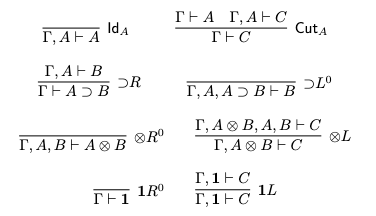
\includegraphics[width=\textwidth]{figures/soprillo.png}
\end{figure}
\end{frame}

\begin{frame}{Cut-Elimination in SAX}
\textbf{Cut elimination fails} because axioms introduce formulas that can't be
decomposed:
\[\tiny
  \infer[{\supset}R]{A \supset B, B \supset C \vdash A \supset C}{
    \infer[\text{Cut}_B]{A, A \supset B, B \supset C \vdash C}{
      \infer[{\supset}L^0]{A, A \supset B \vdash B}{} &
      \infer[{\supset}L^0]{B, B \supset C \vdash C}{}
    }
  }
\]
But this cut is \textbf{analytic} $\implies$ subformula property is not lost.    
\end{frame}

\begin{frame}{Snips}
\scriptsize
\textbf{Snips} are cuts where the cut formula is \emph{eligible}, i.e. it arose
as a subformula inside an axiom's principal formula. Eligibility is tracked by
labeling formula occurrences as eligible ($^*$) or irrelevant ($^0$) and
propagating through the derivation
\[
  \infer[\Text{Snip}_A^1]{\Gamma \vdash z : C}{
    \Gamma \vdash x^* : A &
    \Gamma, x : A \vdash z : C
  }
  \;\;\;\;\;
  \infer[\Text{Snip}_A^2]{\Gamma \vdash z : C}{
    \Gamma \vdash x : A &
    \Gamma, x^* : A \vdash z : C
  }
\]
Example:
\[\tiny
  \infer[{\supset}R]{x:A \supset B, y:B \supset C \vdash z:A \supset C}{
    \infer[\text{Snip}_B]{u^*:A, x:A \supset B, y:B \supset C \vdash w^*:C}{
      \infer[{\supset}L^0]{u^*:A, x:A \supset B, y^0:B \supset C \vdash t^*:B}{} &
      \infer[{\supset}L^0]{u^0:A, x^0:A \supset B, t^*:B, y:B \supset C \vdash w^*:C}{}
    }
  }
\]
\textbf{Cut-free in SAX} = no general cuts, snips permitted $\implies$ 
Admissibility of cut
\end{frame}

\begin{frame}{Labelled Soprillo}
\begin{figure}[H]
  \centering
  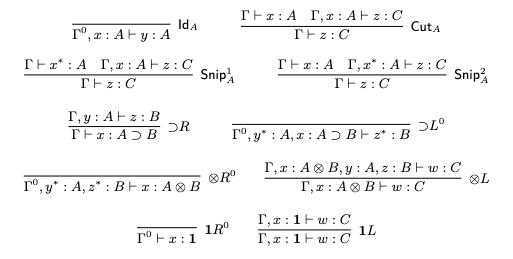
\includegraphics[width=\textwidth]{figures/soprillo-lbl.png}
\end{figure}
\end{frame}


\begin{frame}{Proof Theory: Main Results}

\begin{theorem}[Admissibility of Cut in SAX]
  If there are cut-free derivations of $\Gamma \vdash x : A$ and
  $\Gamma, x : A \vdash z : C$, then there exists a cut-free derivation
  of $\Gamma \vdash z : C$.
\end{theorem}

\begin{theorem}[Cut Elimination in SAX]
  If there is a derivation of $\Gamma \vdash x : A$, then there is a cut-free
  derivation of the same sequent. 
\end{theorem}

\begin{theorem}[Subformula Property]
  All formulas in a cut-free derivation of $\Gamma \vdash x : A$ are
  subformulas of formulas in $\Gamma$ or $A$.
\end{theorem}

\end{frame}


\begin{frame}{Cut Admissibility: A Worked Example}

TODO

\end{frame}


% ===========================================================================
% Arman

\begin{frame}{SAX: Shared Memory Interpretation}
\scriptsize
\textbf{Key idea:} variables become addresses; a sequent
\[
  x_1 : A_1, \ldots, x_n : A_n \vdash P :: (z : C)
\]
types a process $P$ that \textbf{reads} from $x_1, \ldots, x_n$ and \textbf{writes} to $z$.

\medskip
Rules correspond to memory operations:
\begin{itemize}
\item \textbf{Cut} $\to$ allocate a fresh cell (a \emph{future}): $x
  \leftarrow P\,;\,Q$  
\item \textbf{Axioms} $\to$ write;\quad \textbf{Invertible rules} $\to$
  read;\quad \textbf{Identity} $\to$ $\mathtt{copy}\; a\; b$
\end{itemize}

\medskip
\textbf{Example}: ${\supset}L^0$ reads the continuation at $x$,
passing argument $y$ and destination $z$:
\[
  \infer[{\supset}L^0]
    {\Gamma,\, y^*\!:A,\, x : A \supset B \vdash x^R.\langle y, z\rangle :: (z^*\!:B)}{}
\]

\medskip
\textbf{Configurations} are multisets of:
$\mathtt{thread}(a,P)$,\;
% Check the definition of this in the paper, this was wrong I believe
$!\mathtt{cell}(a, W)$,\;
$\mathtt{cell}(c, \_)$ 

\medskip
\textbf{Properties:} Preservation, Progress, Confluence, Termination.
\end{frame}


% ===========================================================================
% Max

\begin{frame}{Mechanizing SAX}

    \begin{itemize}
      \item $G_3$ and Theorems 1 and 2 (cut elim. $G_3$) $\checkmark$ (Pfenning 2000) \textcolor{red}{In LF, not Beluga}
      \item SAX $\checkmark$ , Theorem 3 (translation) $\checkmark$
      \item miniSAX as a subset with $\supset$ only \checkmark) (possibility: extend to $\otimes$)
      \item Eligibility for snips as well-formedness predicate (a la linearity predicate) $\checkmark$
      \item Theorem 5 (cut admissibility) $\checkmark$, Theorem 6 (cut eligibility) should follow
      \item \textcolor{red}{Remaining:} Theorem 7 (Subformula property), configurations required for preservation, progress, etc.
    \end{itemize}
\end{frame}

\begin{frame}

\begin{itemize}
      \item SAX $\checkmark$ , Theorem 3 (translation) $\checkmark$
\end{itemize}

  \scriptsize
\ttfamily

LF hypS : o $\to$ type = ;\\
LF concS : o $\to$ type =\\[4pt]

\quad | initialS : (hypS A $\to$ concS A)\\
\quad | \&RS : concS A $\to$ concS B $\to$ concS (A \& B)\\
\quad | \&L01S : hypS (A \& B) $\to$ concS A\\
\quad | \&L02S : hypS (A \& B) $\to$ concS B\\
\quad | $\supset$RS : (hypS A $\to$ concS B) $\to$ concS (A $\supset$ B)\\
\quad | $\supset$L0S : hypS A $\to$ hypS (A $\supset$ B) $\to$ concS B\\
\quad | $\vee$R01S : hypS A $\to$ concS (A $\vee$ B)\\
\quad | $\vee$R02S : hypS B $\to$ concS (A $\vee$ B)\\
\quad | $\vee$LS : (hypS A $\to$ concS C) $\to$ (hypS B $\to$ concS C) $\to$ (hypS (A $\vee$ B) $\to$ concS C)\\
\quad | cutS : concS A $\to$ (hypS A $\to$ concS C) $\to$ concS C\\
\quad | $\otimes$R0S : hypS A $\to$ hypS B $\to$ concS (A $\otimes$ B)\\
\quad | $\otimes$LS : (hypS A $\to$ hypS B $\to$ concS C) $\to$ (hypS (A $\otimes$ B) $\to$ concS C)\\
\quad | unitRS : concS unit\\
\quad | unitLS : concS C $\to$ (hypS unit $\to$ concS C)\\
;

rec seq2sax : (A : [$\vdash$ o]) rel-ctx-S [$\Gamma$] [$\Gamma'$]
              → [$\Gamma \vdash$ conc A[]] → [$\Gamma' \vdash$ concS A[]] = ...
\end{frame}

\begin{frame}


\begin{itemize}
    \item  miniSAX as a subset with $\supset$ only \checkmark) (possibility: extend to $\otimes$)
\end{itemize}

 { \scriptsize
\ttfamily

LF mhypS : mo $\to$ type = ;\\
LF mconcS : mo $\to$ type =\\[4pt]

\quad | minitialS : (mhypS A $\to$ mconcS A)\\
\quad | m$\supset$RS : (mhypS A $\to$ mconcS B) $\to$ mconcS (A $\supset$ B)\\
\quad | m$\supset$L0S : mhypS A $\to$ mhypS (A $\supset$ B) $\to$ cmoncS B\\
\quad | mcutS : mconcS A $\to$ (mhypS A $\to$ mconcS C) $\to$ mconcS C\\

;}

\pause

Require some way to discuss snips (eligibility) and get rid of $\texttt{mcutS}$ for cut admissability...


\end{frame}


\begin{frame}{}
\begin{itemize}
    \item Eligibility for snips as well-formedness predicate (a la linearity predicate) $\checkmark$ 
\end{itemize}

\begin{columns}

% LEFT COLUMN (your code)
\begin{column}{0.48\textwidth}

\scriptsize
\ttfamily

LF mlhypS : mo $\to$ type = ;\\
LF melig : mlhypS A $\to$ type = ;\\[4pt]

LF mlconcS* : mo $\to$ type =\\[2pt]

\quad \textcolor{blue}{| m$\supset$lL0S : \{h1 : mlhypS A\} \{h2 : mlhypS (A $\supset$ B)\}\\
\quad\quad melig h1 $\to$ mlconcS* B\\[6pt]}

LF mlconcS : mo $\to$ type =\\[2pt]

\quad | mlinitialS : \{h : mlhypS A\} $\to$ mlconcS A\\[2pt]

\quad \textcolor{red}{| mlsnip1S : mlconcS* A $\to$ (mlhypS A $\to$ mlconcS C) $\to$ mlconcS C\\[2pt]}

\quad \textcolor{green}{| mlsnip2S : mlconcS A $\to$ (\{h : mlhypS A\} melig h $\to$ mlconcS C) $\to$ mlconcS C\\[2pt]}

\quad | m$\supset$lRS : (mlhypS A $\to$ mlconcS B) $\to$ mlconcS (A $\supset$ B)\\[2pt]

\quad | mlconcS/* : mlconcS* A $\to$ mlconcS A\\

;

\end{column}

% RIGHT COLUMN (empty for now)
\begin{column}{0.48\textwidth}

% Put your other content here
$$\infer[\textcolor{blue}{\supset L^0}]{\Gamma^0, y^* : A, x : A \supset B \vdash z^* : B}{}$$

$$\infer[\textcolor{red}{\textrm{Snip}^1_A}]{\Gamma \vdash z : C}{\Gamma \vdash x^* : A & \Gamma, x : A \vdash y : C}$$

$$\infer[\textcolor{green}{\textrm{Snip}^1_A}]{\Gamma \vdash z : C}{\Gamma \vdash x : A & \Gamma, x^*: A \vdash y : C}$$
\end{column}

\end{columns}

\end{frame}

\begin{frame}{}
    \begin{itemize}
        \item Theorem 5 (cut admissibility) $\checkmark$, Theorem 6 (cut eligibility) should follow
    \end{itemize}

    \begin{columns}
        \begin{column}{0.48\linewidth}
           
\scriptsize
\ttfamily

rec mcut-admis : \{$\Gamma$: mlctx\} \{A: [$\vdash$ mo]\}\\
\quad [$\Gamma \vdash$ mlconcS A[]]\\
\quad $\to$ [$\Gamma$, x:mlhypS A[] $\vdash$ mlconcS C[]]\\
\quad $\to$ [$\Gamma \vdash$ mlconcS C[]] =\\[4pt]

/ total 1 /\\[4pt]

mlam $\Gamma$ ⇒ mlam A ⇒ fn D ⇒ fn E ⇒\\
case (D, E) of\\[4pt]

\quad $\dots$\\[4pt]

\quad | ([$\Gamma \vdash$ D], [$\Gamma$, x : mlhypS A[] $\vdash$ m$\supset$lRS (\textbackslash h.\ B)]) ⇒\\[4pt]

\quad\quad let [$\Gamma$, z : mlhypS \_ $\vdash$ F] = mcut-admis \_ \_\\
\quad\quad\quad [$\Gamma$, z : mlhypS \_ $\vdash$ D[..]]\\
\quad\quad\quad [$\Gamma$, z : mlhypS \_, x : mlhypS A[] $\vdash$ B[..,z]]\\
\quad\quad in\\[4pt]

\quad\quad [$\Gamma \vdash$ m$\supset$lRS (\textbackslash h.\ F[..,h])]\\[4pt]

\quad $\dots$\\

;
        \end{column}

        \begin{column}{0.48\linewidth}
            \resizebox{\linewidth}{!}{$$\infer[\textrm{Cut}_A]{\Gamma \vdash C_1 \supset C_2}{\deduce{\Gamma \vdash x : A}{\mathcal{D}} & 
            \infer[\supset R]{\Gamma, x : A \vdash z : C_1 \supset C_2}{\deduce{\Gamma, x : A, z_1 : C_1 \vdash z_2 : C_2}{\mathcal{E}}}}$$}
            
            $$\Longrightarrow$$
            \resizebox{\linewidth}{!}{
            $$\infer[\supset R]{\Gamma \vdash z : C_1 \supset C_2}{\infer[IH]{\Gamma, z_1 : C_1 \vdash z_2 : C_2}{\deduce{
            \Gamma, z_1^0 : C_1 \vdash x : A}{\mathcal{D} + \{z_0^1 : C_1\}}
            &\deduce{
            \Gamma, x : A, z_1 : C_1 \vdash z_2 : C_2}{\mathcal{E}_0}
            }}$$}
        \end{column}
    \end{columns}
\end{frame}


\begin{frame}{}
    \begin{itemize}
        \item \textcolor{red}{Remaining:} Theorem 7 (Subformula property), configurations required for preservation, progress, etc.
    \end{itemize}
\end{frame}


\begin{frame} {Related Work}
    \begin{itemize}
        \item Francalaza et. al\cite{FrancalanzaTP24} Presents an implementation of the message-passing interpretation of SAX in Go. Instead of focusing on a pure implementation, we focus on a mechanization of the meta-theoretic properties.
        \item Zhang et al.\cite{zhang2025} gives a mechanization of logical relations for message passing protocols in Coq.
        \item DeYoung et al.\cite{DeYoungP23} presents several metatheoretic proofs for SNAX, including type-safety.
    \end{itemize}

\end{frame}

\begin{frame}{Timeline}
  \begin{itemize}
    \item Mechanize statics and dynamics - March 13th
    \item Mechanize subformula property, begin slides - March 18th
    \item Mechanize Admissibility of cut, cut-elimination, begin initial stages of writeup - March 25th
    \item Finish slides - April 4th
    \item Mechanize type preservation, confluence, Progress - April 10th
    \item Mechanize termination, SNAX, finish writeup - mid April
  \end{itemize} 
\end{frame}

\bibliographystyle{plain}
\bibliography{main}

\end{document}